\chapter{MicroMundo: Análisis y Desarrollo}
  \section{Análisis}
    \subsection{El ecósistema como un sistema complejo}
      Un ecosistema por si mismo es un sistema complejo. Se encuentra compuesto por organismos vivos en un hábitad determinado. Plantas y animales son componentes bióticos de un ecosistema, mientras qué el agua, aire, temperatura, luz, clima y lluvias son componentes abióticos.

      Tanto los componentes bióticos como abióticos forman relaciones entre ellos que caracterízan al ecosistema como tal brindando un balance ``temporal''. De acuerdo a sus tareas dentro del ecosistema, los componentes bióticos pueden ser divididos en:

      \begin{itemize}
        \item \textbf{Productores}: Los organismos autótrofos que producen por si mismos materia orgánica que necesitan para vivir y crecer utilizando moléculas inorgánicas como agua, dióxido de carbono y nitratos, en ésta área podemos encontrar plantas, algas y algúnas bacterias.
        \item \textbf{Consumidores}: También conocidos como organismos heterótrofos, debido a que no pueden producir su propio alimento, sin embargo, pueden alimentarse o bien alimentar también a los productores (por medio de desechos orgánicos o heces fecales).
        \item \textbf{Descomponedores}: Bien son bacterias que se dedican a descomponer la materia orgánica de los tejidos u organismos muertos y regresan las moléculas al ambiente.
      \end{itemize}     

      Cada ecosistema contiene una cantidad dada de materia orgánica que incluye tanto vegetales como animales, el conjunto o peso de todos los componentes se le conoce como biomasa.\cite{6}

      La relación entre los componentes mencionados es algo fundamental en el área de biología. Los ecosistemas, y ciertamente la biosfera global son prototipos de sistemas adaptativos complejos, en donde las propiedades su sistema macroscópico, como su estructura trófica (Cadena alimentícia), diversidad y productividad, patrones y flujo de nutrientes, surge de la interacción entre los componentes y ésta retroalimenta al sistema para seguir generando las relaciones antes mencionadas.      

      Indudablemente, los ecosistemas muestran regularidades en estructura y funcionalidad a través de las regiones, esto extiende los patrones de la distribución de los ecosistemas hasta las variables físicas, cómo el clima de la región y características del suelo. \cite{7}

      \begin{figure}[h!]
        \centering
          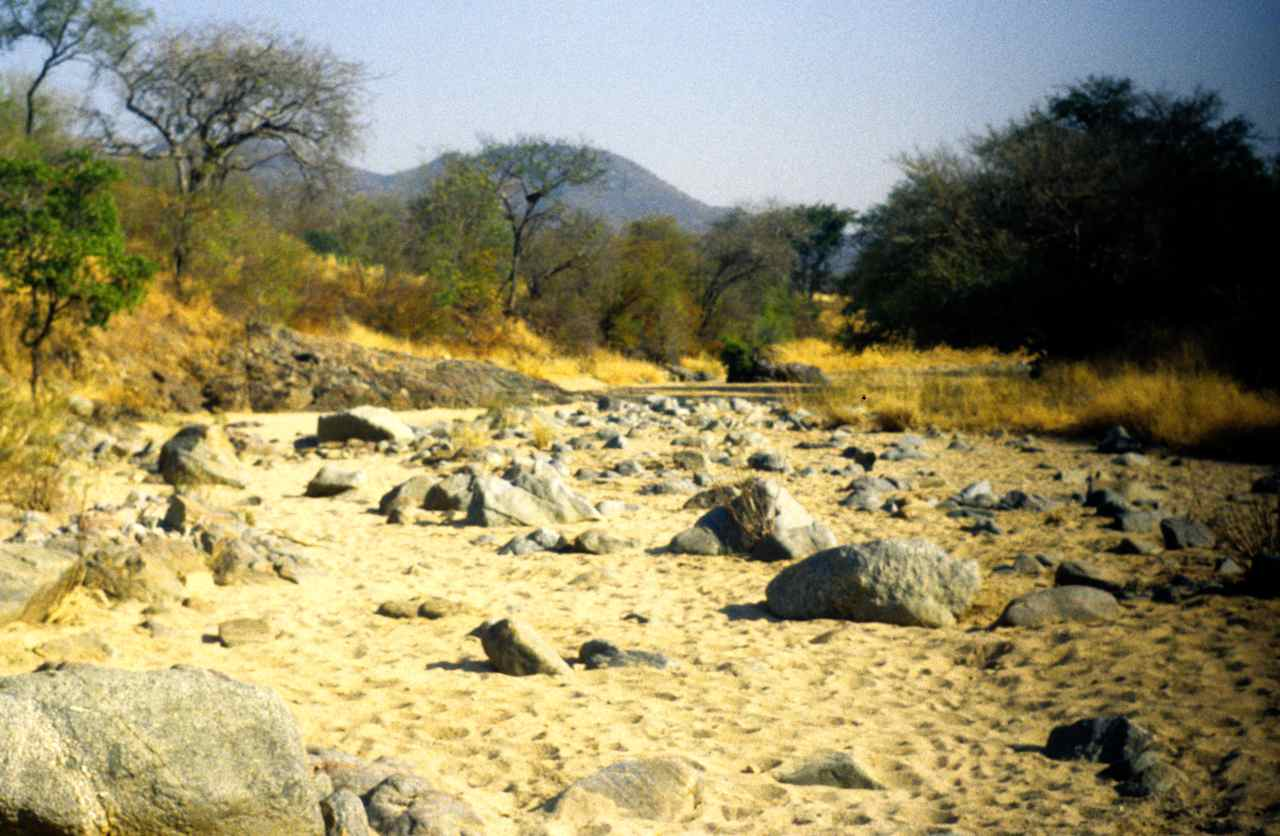
\includegraphics[width=\textwidth]{./images/Ecosistema}
          \caption{Ecosistema semi desértico.} 
      \end{figure}

      Los sistemas complejos han ayudado a la comprensión de la ecología en muchas áreas, por ejemplo, en las fluctuaciónes de la población de un área dada. Esto ha sido logrado debido al análisis de los individuos y el modelado de simples métricas que permiten la convivencia de éstos en un ambiente dado.

      El comportamiento emergente de un ecosistema puede ser variado. Por ejemplo, la competencia y cooperación entre especies hace que éstas se adapten mejor a ciertos obstáculos naturales; también la evolución puede ser vista como un proceso emergente de la interacción, cooperación y competencia entre las especies.

      Una forma de modelar los ecosistemas es mediante agentes basados en objetivos. La meta de los agentes basados en objetivos es diseñar modelos lo suficientemente simples tales que los datos que emergen, puedan ser entendidos y puedean generar entonces un comportamiento más fácil de analizar.

      Los algoritmos genéticos son un ejemplo; éstos fueron diseñados para capturar la esencia de la evolución y adaptación y ser lo suficientemente simples para ser matemáticamente tratables. En los algoritmos genéticos se estudia la evolución de cadenas de símbolos en lugar de intentar simular el comportamiento real de los organismos. \cite{8}